\documentclass{article}
\usepackage{graphicx,amsmath,upquote,lineno,setspace,fullpage}
%\usepackage[square,numbers,sort]{natbib}
\usepackage{natbib}
\addtolength{\textwidth}{0.2in}
\title{Statistical models for point-counting data}
\author{Pieter Vermeesch\\Department of Earth Sciences\\
  University College London\\\texttt{p.vermeesch@ucl.ac.uk}
}
\begin{document}

\linenumbers
\doublespacing

\maketitle

\begin{abstract}
  Point-counting data are a mainstay of petrography,
  micropalaeontology and palynology.  Conventional statistical
  analysis of such data is fraught with problems. Commonly used
  statistics such as the arithmetic mean and standard deviation may
  produce nonsensical results when applied to point-counting data.
  This paper makes the case that point-counts represent a distinct
  class of data that requires different treatment. Point-counts are
  affected by a combination of (1) true compositional variability and
  (2) multinomial counting uncertainties. The relative significance of
  these two sources of dispersion can be quantified by a chi-square
  statistic and -test.  For datasets that pass the chi-square test for
  homogeneity, the `pooled' composition is shown to represent the
  optimal estimate for the underlying population. It is obtained by
  simply adding together the counts of all samples and normalising the
  resulting values to unity. However, more often than not,
  point-counting datasets fail the chi-square test. The overdispersion
  of such datasets can be captured by a random effects model that
  combines a logistic normal population with the usual multinomial
  counting uncertainties.  This gives rise to the concept of a
  `central' composition as a more appropriate way to average
  overdispersed data.  Two- or three-component datasets can be
  displayed on radial plots and ternary diagrams, respectively. Higher
  dimensional datasets may be visualised and interpreted by
  Correspondence Analysis (CA). This is a multivariate ordination
  technique that is similar in purpose to Principal Component Analysis
  (PCA). CA and PCA are both shown to be special cases of
  Multidimensional Scaling (MDS). Generalising this insight to
  multiple datasets allows point-counting data to be combined with
  other data types such as chemical compositions by means of 3-way
  MDS.  All the techniques introduced in this paper have been
  implemented in the \texttt{provenance} \texttt{R}-package, which is
  available from \texttt{http://provenance.london-geochron.com}.
\end{abstract}

\section{Introduction}
\label{sec:intro}

The mineralogical composition of silicilastic sediments can be
determined by tallying the occurrence of various minerals in a
representative sample of (200-400, say) grains \citep{dryden1931,
  vanderplas1965, weltje2002}. Similarly, the fossil content of a deep
sea sediment core may be characterised by tabulating the relative
abundances of various species among $>$100 randomly selected specimens
\citep{patterson1989, buzas1990, fatela2002}. Or palaeobiological
environments may be reconstructed by tabulating the relative frequency
of different types of pollen in a palaeosol or charcoal
\citep{barkley1934, clark1982, weng2006}.\\

These are all examples of multivariate counting experiments, in which
the unknown proportions of different species of minerals, fossils or
pollen are estimated by counting a finite number of randomly selected
items from a representative sample. Despite the widespread use of this
type of data in the Earth Sciences and related fields, their
statistical analysis is demonstrably underdeveloped.\\

For example, there currently exists no agreed method to average
multi-sample point-counting datasets, or to quantify point-counting
data dispersion. Traditionally, these operations were done by taking
the arithmetic mean and standard deviation, respectively.
Unfortunately, this may easily produce nonsensical results. For
example, \citet{weltje2002} shows that the common practice of using
`2-sigma' confidence bounds around the arithmetic mean can produce
physically impossible negative values when applied to petrographic
point-counts.\\

To solve these problems, \citet{weltje2002} argues that point-counts
should be treated as \emph{compositional} data, which are defined as
``vectors representing parts of a whole that only carry relative
information'' \citep{pawlowsky2011}.  According to this definition,
compositional data can be renormalised to a constant sum (e.g., 100\%
if the composition is expressed as percentages, or 1 if fractions are
used) without loss of information. \citet{aitchison1982,
  aitchison1986} shows that the statistical analysis of such data is
best carried out using a simple logratio transformation.\\

To illustrate this approach, let $\left\{a_i, b_i, c_i\right\}$ be a
three-component dataset, where $a_i + b_i + c_i = 1$ for $1 \leq i
\leq m$. Then this dataset can be mapped to a bivariate Euclidean data
space as follows:

\begin{equation}
  u_i = \ln(a_i/c_i) \mbox{~and~} v_i = \ln(b_i/c_i)
  \label{eq:alr}
\end{equation}

After performing the desired statistical analysis (such as calculating
averages and confidence regions) on the transformed data
$\left\{u_i,v_i\right\}$, the results can be mapped back to the
ternary diagram by means of an inverse logratio transformation:

\begin{equation}
  \begin{split}
  a_i & = \frac{\exp[u_i]}{\exp[u_i] + \exp[v_i] + 1} \mbox{,}\\
  b_i & = \frac{\exp[v_i]}{\exp[u_i] + \exp[v_i] + 1} \mbox{, and}\\
  c_i & = \frac{1}{\exp[u_i] + \exp[v_i] + 1}
  \end{split}
  \label{eq:ialr}
\end{equation}

This procedure yields geologically meaningful (geometric) means and
confidence regions. \citet{weltje2002}'s adoption of logratio
statistics to point-counting data represents a huge improvement over
the `crude' statistics employed previously. But it does not solve all
our problems.  There are two crucial differences between point counts
and the classical compositional data discussed by
\citet{aitchison1982,aitchison1986}.\\

First, point-counting data are associated with significant (counting)
uncertainties, which are ignored by classical compositional data
analysis. For a single sample, this uncertainty is adequately
described by multinomial counting statistics \citep[Section~6
  of][]{weltje2002}. But for larger datasets comprised of multiple
samples, existing procedures to construct confidence regions \citep[as
  discussed in Section~7 of][]{weltje2002} are inadequate because they
lump together the `observational' dispersion caused by counting
statistics and the true `geological' dispersion. \citet{bloemsma2015}
describe a method to disentangle these two sources of uncertainty in a
logratio context. They show that deconvolution of (spectroscopic)
count data into a scale vector and a proportions matrix significantly
improves multivariate analysis.\\

Second, point-counting data often contain zero values, which are
incompatible with the log-ratio transformation defined in
Equation~\ref{eq:alr}. This problem also applies to the aforementioned
approach by \citet{bloemsma2015}. These authors circumvented the
occurrence of sporadic zeros by replacing them with small positive
numbers. This and alternative `imputation' strategies are further
discussed by \citet{martin2003}. When the number of zeros is small,
imputation is considered to have a minimal influence on the data
covariance structure.  However, some point-counting datasets are
dominated by zeros. So the presence of such values is not a cosmetic
problem, but a fundamental characteristic of this particular data
type. The statistical treatment of point-counting data needs to
address this issue at a deeper level.\\

The present paper solves these long standing problems using
established statistical methods adopted from other disciplines. Much
of the paper is based on the work of \citet{galbraith2005} in fission
track geochronology. The fission track method is based on the ratio of
the number of spontaneous \textsuperscript{238}U-tracks to the number
of neutron-induced \textsuperscript{235}U-tracks per unit area in
accessory minerals such as apatite or zircon. This is equivalent to a
simple two-component point-counting problem. Section~\ref{sec:pooled}
uses this equivalence to derive the concept of a `pooled
composition'. We will show that the latter represents the most
reliable (in terms of accuracy and precision) average of homogeneous
point-counting data.\\

The analytical uncertainty of individual point-counting proportions
may greatly vary between samples. Section~\ref{sec:radial} introduces
\citet{galbraith1988}'s radial plot as a graphical means of
visualising such `heteroscedastic' data. Originally developed for
fission track data, the radial plot can also be used to display
point-counting ratios, which frequently occur in the Earth
Sciences. Radial plots allow a visual assessment of the degree to
which counting uncertainties can explain the observed scatter between
multiple ratio estimates. Section~\ref{sec:X2} presents a formal
statistical test to make this assessment more quantitative.\\

The pooled composition is only applicable to samples that pass this
chi-square test for sample homogeneity.  Multi-sample datasets that
fail the chi-square test are said to be `overdispersed' with respect
to the counting uncertainties. The degree of overdispersion may be
quantified by means of a continuous mixture model
(Section~\ref{sec:randomeffects}). This model leads to the concept of
a `central composition' as a better alternative to the pooled
composition of Section~\ref{sec:pooled}.  Section~\ref{sec:ternary}
generalises the continuous mixture model from two to three (or more)
components.\\

Finally, Section~\ref{sec:CA} introduces Correspondence Analysis (CA)
as a useful ordination technique for multivariate point-counting
data. CA is closely related to compositional Principal Component
Analysis (PCA). But unlike the latter method, it does not suffer from
the zero counts problem.\\

All the techniques discussed above will be illustrated with a
combination of synthetic and real examples. The methods of
Sections~\ref{sec:pooled}-\ref{sec:ternary} will use the two datasets
shown in Table~\ref{tab:data}. Data~1 consists of 20 random samples of
23--94 items each, which were drawn from a discrete trinomial
distribution with 45\% of component $a$, 45\% of component $b$ and
10\% of component $c$.  Data~2 comprises a further 20 samples that
were drawn from a continuous distribution whose mode is the same as
that of Data~1, but which adds 100\% of dispersion around this
mode. Thus, Data~2 has two sources of dispersion (counting error and
true population dispersion), whereas Data~1 only has one (counting
error). Note that both datasets contain fewer counts per sample than
is customary in real world applications. But they are nevertheless
realistic if we consider them to be ternary subcompositions of higher
dimensional datasets.\\

\begin{table}[!ht]
  \centering
  \begin{tabular}{c|ccc|c||c|ccc|c}
\multicolumn{5}{c||}{Data~1} & \multicolumn{5}{c}{Data~2} \\ \hline
\#& $a$& $b$& $c$& $R$& \#& $a$& $b$& $c$& $R$ \\ \hline
1& 16& 18& 4& 38& 1& 23& 24& 5& 52 \\
2& 25& 17& 3& 45& 2& 60& 24& 7& 91 \\
3& 18& 18& 0& 36& 3& 45& 43& 12& 100 \\
4& 7& 14& 3& 24& 4& 2& 53& 4& 59 \\
5& 12& 10& 3& 25& 5& 8& 32& 10& 50 \\
6& 32& 30& 13& 75& 6& 53& 21& 23& 97 \\
7& 35& 38& 13& 86& 7& 1& 6& 3& 10 \\
8& 20& 20& 7& 47& 8& 2& 17& 1& 20 \\
9& 10& 9& 3& 22& 9& 10& 10& 4& 24 \\
10& 29& 36& 5& 70& 10& 2& 35& 3& 40 \\
11& 34& 34& 9& 77& 11& 29& 21& 3& 53 \\
12& 22& 47& 12& 81& 12& 2& 13& 0& 15 \\
13& 9& 9& 2& 20& 13& 3& 9& 0& 12 \\
14& 37& 36& 13& 86& 14& 34& 1& 0& 35 \\
15& 46& 25& 16& 87& 15& 28& 19& 4& 51 \\
16& 50& 37& 7& 94& 16& 49& 11& 3& 63 \\
17& 28& 34& 8& 70& 17& 0& 72& 2& 74 \\
18& 39& 50& 6& 95& 18& 55& 28& 13& 96 \\
19& 44& 36& 10& 90& 19& 7& 8& 3& 18 \\
20& 28& 21& 4& 53& 20& 20& 5& 2& 27 \\
\hline
$C$& 541& 539& 142& $N=1222$& $C$& 433& 452& 90& $N=987$
  \end{tabular}
  \label{tab:data}
  \caption{Two synthetic ternary point-counting datasets.  Data~1 was
    drawn from a single multinomial distribution with population
    proportions of 45\%, 45\% and 10\% for components $a$, $b$ and
    $c$, respectively. Data~2 was drawn from a continuous mixture of
    multinomial distributions whose true proportions were drawn from a
    bivariate logistic normal distribution with a geometric mean of
    45\% for $a$ and $b$, 10\% for $c$, and 100\% dispersion with a
    correlation coefficient of -0.5 between the two logratio
    dimensions. $R$, $C$ and $N$ refer to the row, column, and total
    sums, respectively.}
\end{table}

\section{The pooled composition}
\label{sec:pooled}

Let us partition a population of objects (such as minerals, fossils or
pollen) into two classes. Let $\theta$ be the true fraction of the
first class, and $(1-\theta)$ the true fraction of the second class,
respectively. Suppose that we have collected $m$ representative
samples of randomly selected items from this population. For each of
these samples, let $n_{i1}$ represent the number of items belonging to
the first class and $n_{i2}$ the number of items belonging to the
second class (for $1 \leq i \leq m$). Further let $n_{i\bullet}$ be
the total number of counts in the $i$\textsuperscript{th} sample so
that $n_{i\bullet} \equiv n_{i1} + n_{i2}$. The probability of
observing $n_{i1}$ and $n_{i2}$ given $n_{i\bullet}$ then follows a
binomial distribution:

\begin{equation}
  p(n_{i1},n_{i2}|n_{i\bullet}) =
  \binom{n_{i\bullet}}{n_{i1}} \theta^{n_{i1}}
  (1-\theta)^{n_{i2}}
  \label{eq:pnN}
\end{equation}

The true value of $\theta$ is unknown but can be estimated (as
$\hat{\theta}$) by jointly considering all $m$ samples and maximising
their summed log-likelihood ($\mathcal{L}_p$):

\begin{equation}
  \begin{split}
  \mathcal{L}_p = & \sum\limits_{i=1}^{m}
  \left[
    \ln\binom{n_{\bullet i}}{n_{i1}} + n_{i1} \ln(\theta) + n_{i2} \ln(1-\theta)
    \right] \\
  ~ = & \mathrm{~constant} + n_{\bullet 1} \ln(\theta) +
  n_{\bullet 2} \ln(1-\theta)
  \end{split}
  \label{eq:Lpooled}
\end{equation}

\noindent where $n_{\bullet 1} \equiv \sum_{i=1}^{m} n_{i1}$ and
$n_{\bullet 2} \equiv \sum_{i=1}^{m}
n_{i2}$. Equation~\ref{eq:Lpooled} is maximised if $\hat{\theta} =
n_{\bullet 1}/(n_{\bullet 1}+n_{\bullet 2})$.  In other words, the
maximum likelihood solution is found by \emph{pooling} all the counts
together. A $100(1-\alpha)\%$ confidence interval for $\theta$ is
given by:

\begin{equation}
  \frac{n_{\bullet 1}}{ n_{\bullet 1} +
    (n_{\bullet 2}+1) F^{\alpha}_{2(n_{\bullet 2}+1),2n_{\bullet 1}}
  }
  <
  \theta
  <
  \frac{(n_{\bullet 1}+1) F^{\alpha}_{2(n_{\bullet 1}+1),2n_{\bullet 2}}}
       {n_{\bullet 2} + (n_{\bullet 1}+1) F^{\alpha}_{2(n_{\bullet 1}+1),2n_{\bullet 2}}}
  \label{eq:pooledCI}
\end{equation}

\noindent where $F^{\alpha}_{a,b}$ denotes the
100(1-$\alpha$)-percentile of an F-distribution with $a$ and $b$
degrees of freedom. The same equation can be used to construct a
confidence interval for $\theta_i$ by replacing $n_{\bullet 1}$ with
$n_{i1}$ and $n_{\bullet 2}$ with $n_{i2}$.\\

Let us consider the binary subcomposition comprised of $a$ and $b$ in
samples~11 and 13 of Data~1 as an example. For sample~11, $a = b = 34$
so that $\hat{\theta} = 0.5 \pm 0.11$.  For sample~13, $a = b = 9$ so
that $\hat{\theta} = 0.5 \pm 0.21$.  In other words, although the
binomial parameter estimates of these two samples are the same, the
width of their 95\% confidence intervals differ by a factor of two. In
statistical terms, this is called \emph{heteroscedasticity}. The
following section of this paper will introduce a graphical means of
visualising such data.

\section{A radial plot for point-counting ratios}
\label{sec:radial}

In many Earth Sciences applications, it is not so much the absolute
proportions but the ratios between binary (sub)compositions that are
of interest. For example, in the context of heavy mineral analysis the
apatite/tourmaline, monazite/zircon, and TiO\textsubscript{2}/zircon
ratios \citep[e.g.,][]{morton1994}, and the epidote/garnet ratio
\citep{heroy2003} have all be used to indentify the provenance of
sediments. In micropalaeontology, the ratio of benthic to planktonic
foraminifera has been used as a productivity index
\citep[e.g.,][]{berger1988}. And in palynology, the
arboreal/non-arboreal pollen ratio is widely used as an index of
landscape openness \citep[e.g.,][]{herzschuh2007}.\\

Given an estimate of the binomial parameter, $\hat{\theta}$, such
ratios can be simply obtained as $\hat{\theta}/(1-\hat{\theta})$.  The
corresponding $100(1-\alpha)\%$ confidence intervals can be calculated
using Equation~\ref{eq:pooledCI}. Applying this to samples~11 and 13
of Data~1 as an example, we obtain $a/b$-ratio estimates of 1.00
+0.53/-0.35 for for sample~11, and 1.00 +1.43/-0.58 for sample~13.  So
like the binomial parameter estimates, also the ratio estimates are
heteroscedastic. A radial plot is a graphical device that was
specifically designed to display such data.\\

Given a set of paired counts $\left\{n_{i1},n_{i2}\right\}$ (for $1
\leq i \leq m)$, the radial plot is a scatter diagram that sets out
$(z_i-z_\circ)/s_i$ against $1/s_i$, where

\begin{equation}
  \begin{split}
    z_i & = \arcsin\left(\sqrt{(n_{i1}+3/8)/(n_{i\bullet}+3/4)}\right) ,\\
    z_\circ & = \arctan\left(\sqrt{n_{\bullet 1}/n_{\bullet 2}}\right)
    \mbox{,~and}\\
    s_i & = 1 / \left(2 \sqrt{n_{i\bullet}+1/2}\right)
  \end{split}
  \label{eq:radial}
\end{equation}

Precise measurements plot towards the right hand side of this plot and
imprecise measurements to the left. The actual $n_{1i}/n_{2i}$-ratio
is proportional to the slope of a line connecting the
$i$\textsuperscript{th} data point to the origin. The corresponding
values are shown on a circular scale shown at some convenient radial
distance away from the origin.\\

Figure~\ref{fig:radial}.i shows a radial plot for the first two
components ($a$ and $b$) of Data~1.  Samples~11 and 13 of Data~1 have
been highlighted. Recall that the estimated $a/b$-ratio of sample~11
has the same value but twice the precision of sample~13. Therefore,
sample~11 plots at the same angle, but towards the right of
sample~13.\\

Figure~\ref{fig:radial}.ii displays the $a/b$-ratios of Data~2. Let us
have a closer look at samples~2 and 7, which are marked in black on
this diagram. The total number of grains counted in these two samples
are $n_{2\bullet} = 60 + 24 = 84$, and $n_{7\bullet} = 1 + 6 = 7$,
respectively (Table~\ref{tab:data}). So sample~2 is twelve times
larger than sample~7, allowing a more precise $a/b$-ratio estimate.
Sample~2 therefore plots to the right of sample~7, causing the
95\%-confidence interval for the former sample to be narrower than
that of the latter.  Projecting the two samples onto the radial scale
yields a ratio of $a/b = 2.5 +1.7/-1.0$ for sample~2 and $a/b = 0.17
+1.20/-0.16$ for sample~7.\\

The dispersion of the data with respect to the counting uncertainties
can be visually assessed by comparing the vertical scatter of the data
with a confidence band of two standard errors wide drawn on either
side of the origin.  If approximately 95\% of the data plot within
this interval, then the data are compatible with a homogeneous
composition. This is the case for Data~1, which can therefore be
safely averaged using the pooled ratio (Figure~\ref{fig:radial}.i).
In contrast, the $a/b$-ratios of Data~2 significantly scatter beyond
the `2-sigma' confidence region (Figure~\ref{fig:radial}.ii). In this
case the pooled average should be abandoned in favour of a
heterogeneous model (Section~\ref{sec:randomeffects}).\\

In conclusion, the radial plot is a useful device to visually assess
the dispersion of point-counting ratios. The next section of this
paper introduces a formal statistical test to make this assessment
more quantitative.

\begin{figure}[!ht]
  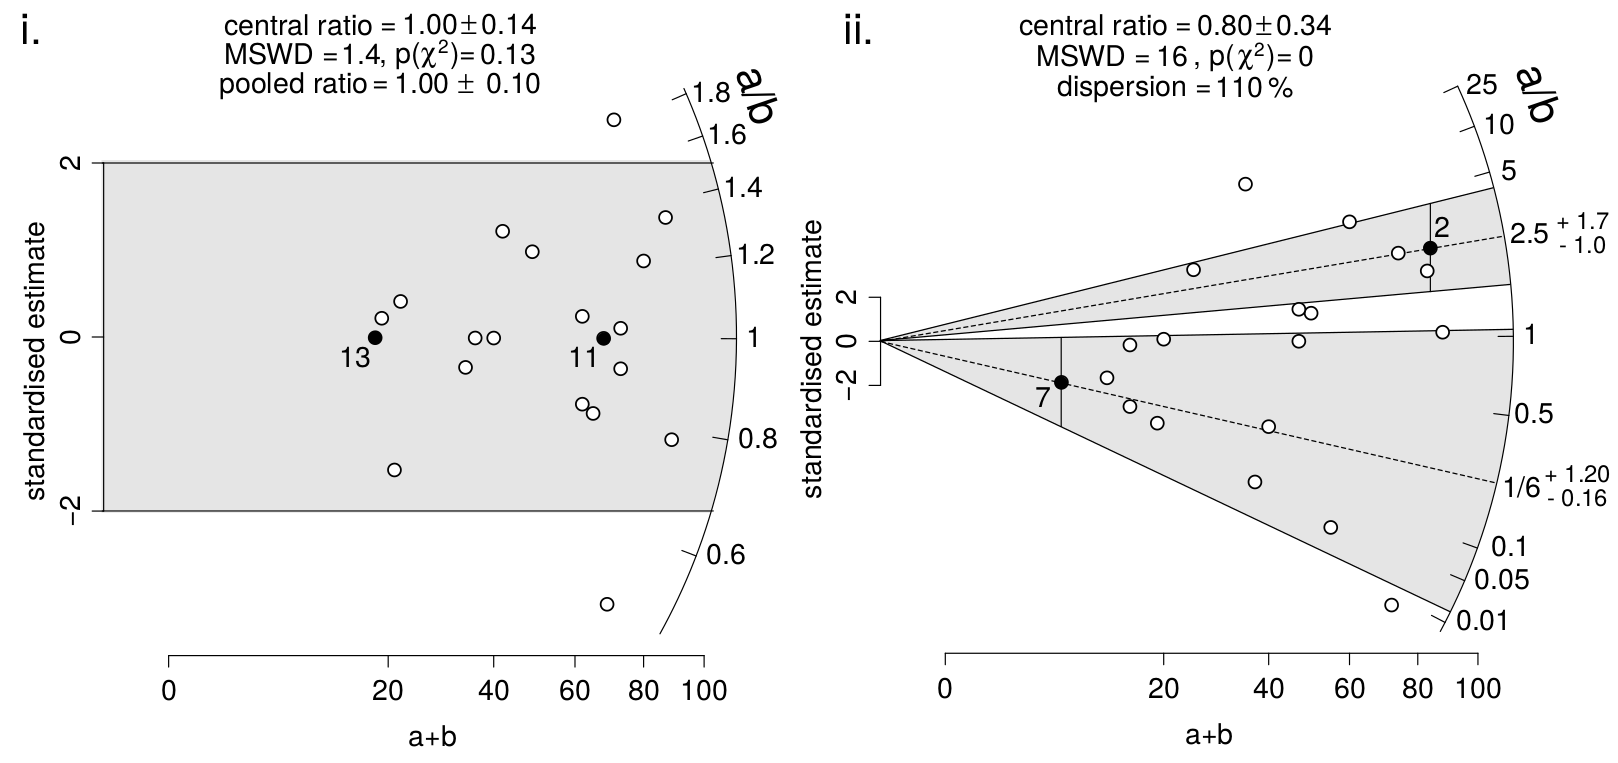
\includegraphics[width=\textwidth]{radialplots.png}
  \caption{Radial plots of the binary subcompositions $a$ and $b$ for
    Table~\ref{tab:data}.  i) approximately 95\% of the samples in
    Data~1 plot within a symmetric `2-sigma' band around the
    origin. These data are therefore compatible with a single
    homogeneous population. The pooled composition then is the best
    estimate for the average composition (Section~\ref{sec:pooled}).
    ii) the $a/b$-ratio of each sample can be obtained by projecting
    the corresponding scatter point onto the radial scale.  The black
    dots mark samples~2 (right) and 7 (left) of Data~2. Projecting a
    `2-sigma' error bar onto the same scale yields the 95\% confidence
    intervals of $a/b = 2.5 +1.7/-1.0$ for sample~2 and $a/b = 0.17
    +1.20/-0.16$ for sample~7, respectively. In contrast with Data~1,
    the $a/b$-ratios of Data~2 do not fit within a `2-sigma' band.  In
    this case the data are more adequately described by a random
    effects model with two parameters: the central ratio and the
    dispersion.}
  \label{fig:radial}
\end{figure}

\section{A chi-square test for compositional homogeneity}
\label{sec:X2}

In order for the pooled composition to be a meaningful description of
the detrital population, all samples must be derived from a single
true composition. In other words, any observed differences in the
$n_{i1}/n_{i2}$-ratios must be due to binomial counting statistics
alone. The validity of this assumption can be verified by calculating
the chi-square statistic:

\begin{equation}
  \chi_{stat}^{2} = \frac{1}{n_{\bullet 1} n_{\bullet 2}}
  \sum\limits_{i=1}^{m}
  \frac{\left[n_{i1}n_{\bullet2}-n_{i2}n_{\bullet 1}\right]^2}{n_{i\bullet}}
  \label{eq:X2}
\end{equation}

If $\chi_{stat}^2$ is greater than the $100(1-\alpha)$-percentile of a
chi-square distribution with ($m-1$) degrees of freedom, then the null
hypothesis of compositional homogeneity is rejected on a
$100(1-\alpha)\%$ confidence level, where $\alpha$ is usually taken to
be 0.05.\\

An alternative way to quantify the dispersion of the data with respect
to the expected counting fluctuations is to divide $\chi_{stat}^2$ by
the number of degrees of freedom. This parameter is known as the
`reduced chi-square statistic', but is also frequently referred to as
the `Mean Square of the Weighted Deviates' in the Earth Sciences
\citep{wendt1991}:

\begin{equation}
  \mbox{MSWD} \equiv \chi_{stat}^2/(m-1)
\end{equation}

If the observed scatter is entirely due to binomial counting
statistics, then the MSWD is expected to take values close to unity.
This is the case for Data~1, which is characterised by an MSWD of 1.4
and a p-value of 0.13. The latter value is well above the 0.05 cutoff,
making the pooled composition the most appropriate average. The pooled
$a/b$-ratio of Data~1 is 1.00 $\pm$ 0.10, which agrees with the known
ratio of 1.00 (Section~\ref{sec:intro}).\\

MSWD values significantly greater than one indicate the presence of
excess scatter beyond the binomial counting statistics.  This is the
case for Data~2, which yields an MSWD-value of 16 and a p-value close
to zero. In this situation, the pooled average is not the most
appropriate estimator for the population average and a more realistic
model must be used. An example of one such model is given in
Section~\ref{sec:randomeffects}.

\section{Continuous mixtures}
\label{sec:randomeffects}

Datasets that fail the chi-square test for homogeneity are
incompatible with a single binomial population. Instead their binomial
population parameter $\theta$ may be drawn from a continuous
distribution. Suppose that $\theta$ is drawn from a logistic normal
distribution with geometric mean $\mu$ and coefficient of variation
$\sigma$, and define

\begin{equation}
  \beta \equiv \ln\left(\frac{\theta}{1-\theta}\right)
  \sim \mathcal{N}(\mu,\sigma^2)
  \label{eq:logTheta}
\end{equation}

\noindent where $\mathcal{N}(\mu,\sigma^2)$ stands for ``the normal
distribution with mean $\mu$ and variance $\sigma^2$''. Note that
$\beta$ is a logratio similar to those defined in
Equation~\ref{eq:alr}. Given the usual $m$ sets of point-counts
$\{n_{i1},n_{i2}\}$ and maximising the log-likelihood function
$\mathcal{L}_c$

\begin{equation}
  \mathcal{L}_c = \sum\limits_{i=1}^{m}\ln\left\{
  \binom{n_{i\bullet}}{n_{i1}}
  \int\limits_{-\infty}^{\infty}
  \frac{\exp\left[\beta n_{i1}\right]}
       {\left(\exp\left[\beta\right] + 1\right)^{n_{i\bullet}}}
  \frac{\exp\left[
         -\frac{1}{2}\left(\frac{\beta-\mu}{\sigma}\right)^2
         \right]}
       {\sigma\sqrt{2\pi}}
       d\beta\right\}
\label{eq:LLbivariatecentral}
\end{equation}

\noindent yields two estimates $\hat{\mu}$ and $\hat{\sigma}$ whose
approximate standard errors may be obtained by inverting the Hessian
matrix of second derivatives of $\mathcal{L}_c$. The integrals in
Equation~\ref{eq:LLbivariatecentral} cannot be evaluated analytically,
but a quick numerical solution is provided by
\citet{galbraith1993}. The `central' composition is then defined as:

\begin{equation}
  \hat{\theta} = \frac{\exp[\hat{\mu}]}{\exp[\hat{\mu}] + 1}
\end{equation}

\noindent which is akin to the inverse logratio transformation defined
in Equation~\ref{eq:ialr}. The central $a/b$-ratio for Data~2 is $0.80
\pm 0.34$ (Figure~\ref{fig:radial}.ii), which again agrees with the
true ratio of 1.00 that was reported in Section~\ref{sec:intro}.\\

The dispersion estimate $\hat{\sigma}$ quantifies the geological
variability of the underlying population. This is just as useful a
quantity as the central value itself. It estimates the relative spread
of the underlying population without the binomial counting errors. For
example the coefficient of variation (standard deviation divided by
mean) of the $a/b$-ratio measurements for Data~2 is $\sim$260\%.  This
is far greater than the $\sim$110\% dispersion estimated by the random
effects model. The latter estimate is much closer to the true
dispersion of the underlying population, whose value is 100\%
(Section~\ref{sec:intro}).\\

It is useful to note that, for samples that pass the chi-square test
for sample homogeneity, the pooled ratio is the same as the central
ratio. This is indeed the case for Data~1, which yields a pooled ratio
of 1.00 $\pm$ 0.10 and a central ratio of 1.00 $\pm$ 0.14. The larger
95\% uncertainty interval of the latter is due to the loss of one
degree of freedom that is required to estimate $\hat{\sigma}$.

\section{Ternary models}
\label{sec:ternary}

The statistical models presented in the previous sections can be
generalised from two to three or more components. This is trivial for
homogeneous populations such as Data~1, whose pooled composition is
shown in Figure~\ref{fig:ternarycounts}.i.  For heterogeneous
populations such as Data~2, the continuous mixture model of
Section~\ref{sec:randomeffects} can be generalised by defining two
population parameters $\beta_1 \equiv
\ln[\theta_1]-\ln[1-\theta_1-\theta_2]$ and $\beta_2 \equiv
\ln[\theta_2]-\ln[1-\theta_1-\theta_2]$.  Assuming that $\beta_1$ and
$\beta_2$ are drawn from a bivariate normal distribution with mean $M$
and covariance matrix $\Sigma$, the three-component equivalent to
Equation~\ref{eq:LLbivariatecentral} becomes

\begin{equation}
  \begin{split}
    \mathcal{L}_t =
    \sum\limits_{i=1}^{m}\ln\biggl\{
      \frac{n_{i\bullet}!}{n_{i1}! n_{i2}! n_{i3}!}
      \int\limits_{-\infty}^{\infty}\int\limits_{-\infty}^{\infty}
      \frac{\exp\left[\beta_1 n_{i1} + \beta_2 n_{i2}\right]}
           {\left(\exp\left[\beta_1\right] +
             \exp\left[\beta_2\right] + 1\right)^{n_{i\bullet}}}\\
           \frac{\exp\left[
               -\frac{1}{2}
               \left(B-M\right)^T \Sigma^{-1} \left(B-M\right)
               \right]
           }{
             2\pi\sqrt{|\Sigma|}
           }
           d\beta_1 d\beta_2\biggr\}
  \end{split}
  \label{eq:LLternarycentral}
\end{equation}

\noindent where $\left\{n_{i1},n_{i2},n_{i3}\right\}$ are the ternary
counts of the $i$\textsuperscript{th} sample, with $n_{i1} + n_{i2} +
n_{i3} = n_{i\bullet}$ for $1 \leq i \leq m$;

\begin{equation*}
  B =
  \left[
    \begin{array}{c}
      \beta_1 \\
      \beta_2
    \end{array}
    \right]
  \mbox{;~}
  M =
  \left[
    \begin{array}{c}
      \mu_1 \\
      \mu_2
    \end{array}
    \right]
  \mbox{;~and~}
  \Sigma \equiv
  \left[
    \begin{array}{cc}
      \sigma_1^2 & \sigma_{1,2} \\
      \sigma_{1,2} & \sigma_2^2
    \end{array}
    \right]
\end{equation*}

\noindent  in  which  $\sigma_1$   and  $\sigma_2$  are  the  standard
deviations  of $\beta_1$  and $\beta_2$,  and $\sigma_{1,2}$  is their
covariance.          Equation~\ref{eq:LLternarycentral},          like
Equation~\ref{eq:LLbivariatecentral},  does  not  have  an  analytical
solution and requires numerical integration for each sample.  The fast
algorithm of  \citet{galbraith1993} can  be used to  estimate $\mu_1$,
$\mu_2$,  $\sigma_1$  and  $\sigma_2$  so  that  only  the  covariance
$\sigma_{1,2}$ remains to  be found.  The central  composition is then
estimated by  substituting $\hat{\mu}_1$  for $u_i$  and $\hat{\mu}_2$
for $v_i$ in Equation~\ref{eq:ialr}. Figure~\ref{fig:ternarycounts}.ii
applies this  model to  Data~2, showing the  central composition  as a
black  square  and using  the  dispersion  estimate $\hat{\Sigma}$  to
define a  95\% confidence  region for  the underlying  population (red
line).\\

The definition of $\beta_1$ and $\beta_2$ that is used in
Equation~\ref{eq:LLternarycentral} is consistent with the logratio
approach of Equation~\ref{eq:alr}. However other parameterisations are
possible as well. For example, we could define three logistic
population parameters ($\beta_i \equiv \ln[\theta_i] -
\ln[1-\theta_i]$ for $1 \leq i \leq 3$) to ensure compatibility with
the bivariate random effects model of Section~\ref{sec:randomeffects}.
These alternative parameterisations are interchangeable with each
other and can easily be converted to each other.

\begin{figure}[!ht]
  \centering
  \includegraphics[width=.8\textwidth]{ternarycount.png}
  \caption{Statistical analysis of ternary point-counting
    data. i. Data~1 is sampled from a homogeneous population, whose
    mean is given by the pooled composition shown as a black
    square. ii. Data~2 is derived from a continuous mixture (see the
    caption of Table~\ref{tab:data} for details). Its estimated
    central composition is shown as a black square, and the 95\%
    confidence envelope corresponding to its dispersion parameters as
    a red contour line. The dashed black contour marks the true
    dispersion region for the population, also shown at 95\%
    confidence.}
  \label{fig:ternarycounts}
\end{figure}

\section{Correspondence analysis}
\label{sec:CA}

The previous sections of this paper have shown that binary or ternary
datasets can be visualised as radial plots and ternary diagrams,
respectively. These two-dimensional graphics are useful for
interpreting point-counting data, but cannot so easily be applied to
higher dimensional datasets. In this section, we will consider the
general case of a $K$-component dataset $X$ contained in an $[m \times
  K]$-matrix. We will explore some strategies to display such a
dataset as a two-dimensional graphic.\\

Principal Component Analysis \citep[PCA,][]{pearson1901} is an
ordination techniques that is commonly used for exploratory data
analysis of multi-dimensional datasets.  PCA is a two step
process. First, the data are `centred' by subtracting the arithmetic
mean composition from each column. Second, the centred data are
decomposed into an orthogonal set of $K$ principal components.
Plotting the first two principal components against each other then
yields the desired two-dimensional data projection.\\

Unfortunately, PCA cannot readily be applied to compositional data or
point-counting data. This is because the first step involves taking an
arithmetic mean, which we have already shown to be problematic
in Section~\ref{sec:intro}. Subjecting the data to a logratio
transformation prior to PCA analysis solves this problem
\citep{aitchison1983}. But this solution generally does not work for
point-counting data due to its inability to handle zero count data.
This issue is aggravated by the tendency for high dimensional datasets
to contain more zeros than lower dimensional datasets do.\\

Correspondence Analysis \citep[CA,][]{greenacre1984} fixes these
issues by explicitly treating the data as counts. CA is a multivariate
ordination technique that is conceptually similar to PCA.  To
understand the relationship between the two methods, it is useful to
point out that PCA and CA are both special case of another exploratory
data analysis method called Multidimensional Scaling
\citep[MDS,][]{kruskal1978, vermeesch2013}. Given a table of pairwise
`dissimilarities' between samples, MDS produces a map in which similar
samples plot close together and dissimilar samples plot far apart.\\

PCA is a special case of MDS in which the dissimilarities are
Euclidean distances. CA is another special case of MDS in which the
dissimilarities are chi-square distances \citep{legendre2001,
  greenacre2005}:

\begin{equation}
  d_{ij} =
  \sqrt{
    \sum\limits_{k=1}^K
    \frac{X_{\bullet\bullet}}{X_{\bullet k}}
    \left(\frac{X_{ik}}{X_{i\bullet}} - \frac{X_{jk}}{X_{j\bullet}}\right)^2
  }
  \label{eq:dij}
\end{equation}

\noindent where $d_{ij}$ is the dissimilarity between samples $i$ and
$j$ (with $1 \leq i,j \leq m$); $X_{\bullet k} = \sum_{i=1}^{m}
X_{ik}$; $X_{i\bullet} = \sum_{k=1}^{K} X_{ik}$; $X_{j\bullet} =
\sum_{k=1}^{K} X_{jk}$; and $X_{\bullet\bullet} =
\sum_{i=1}^{m}\sum_{k=1}^{K} X_{ik}$.  In the case of PCA, the
principal components are obtained by linear combination of the
original variables. The weightings of these variables can be displayed
together with the transformed data as a biplot
\citep{aitchison2002}. The same principle can be applied to CA
(Figure~\ref{fig:CA}).

\section{Examples}
\label{sec:examples}

All the methods discussed in this paper were added to the
\texttt{provenance} package of \citet{vermeesch2016a}.  Written in the
statistical programming language \texttt{R}, \texttt{provenance} comes
with a query-based user interface that does not require any
programming skills. Alternatively, the full functionality of the
package can also be accessed via the command line, as demonstrated in
the following tutorial.\\

Point-counting data can be read from a \texttt{.csv} file using the
\texttt{read.counts} function. For example, to read the second dataset
from Table \ref{tab:data}:

\begin{verbatim}
data2 <- read.counts('data2.csv')
\end{verbatim}

Plotting the ratios of the first two variables ($a/b$) as a radial
plot (Figure~\ref{fig:radial}.i):

\begin{verbatim}
radialplot(data2,num='a',den='b')
\end{verbatim}

\noindent where \texttt{num} and \texttt{den} are optional arguments
denoting the names of the numerator and denominator component,
respectively. Plotting the full dataset on a ternary diagram and
constructing its 95\% confidence region
(Figure~\ref{fig:ternarycounts}.ii):

\begin{verbatim}
# create a ternary data object:
tern <- ternary(data2)
# show the data on a ternary diagram
# as white circles without data labels:
plot(tern,pch=1,labels=NA)
# add the 95% confidence region:
ternary.ellipse(tern,alpha=0.05)
\end{verbatim}

\noindent where everything that follows a hash character (`\#') is a
comment and is ignored. Next, let us consider a real dataset of heavy
mineral counts from Namibia published by \citet{vermeesch2016a}.  The
following code snippet calculates the central composition for these
data:

\begin{verbatim}
HM <- read.counts('HM.csv')
avg <- central(HM)
\end{verbatim}

The variable \texttt{avg} contains a $[5 \times 15]$ table in which
each column corresponds to a mineral species, and the rows contain (1)
the central value for the binomial parameters ($\theta_i$ for $1 \leq
i \leq 15$) for those minerals; (2) the standard error for the
binomial parameters; (3) the overdispersion parameter for the binary
composition parameter $\ln[\theta_i]-\ln[1-\theta_i]$; (4) the MSWD
value for each binary subcomposition; and (5) the corresponding
p-value.\\

Next, we will perform a correspondence analysis of the Namib data.
But before doing so, it is important to point out that CA is most
sensitive to the least abundant components.  To mitigate the effects
of this phenomenon, it is useful to pre-process the data. The
following code snippet selects the most abundant minerals (epidote,
garnet, amphibole and clinopyroxene) from the datasets and amalgamates
the ultra-stable minerals (zircon, tourmaline and rutile), which have
similar petrological significance:

\begin{verbatim}
HM2 <- amalgamate(HM,ztr=c('zr','tm','rt'),ep='ep',
                  gt='gt',amp='amp',cpx='cpx')
\end{verbatim}

The resulting data object (\texttt{HM2}) still contains a number
of zero values, but is no longer dominated by them. The actual
CA calculation then proceeds as follows:

\begin{verbatim}
# perform the calculations:
ca <- CA(HM2)
# show the results as a biplot:
plot(ca)
\end{verbatim}

The biplot (Figure~\ref{fig:CA}) displays the samples in black and the
minerals as red arrows. The tight clustering of samples N1, N2, N3,
N10, N12, N14, T8 and T13 reflects the compositional similarity
between these samples, which were all derived from the coastal parts
of the Namib Sand Sea \citep{vermeesch2015}.  In contrast, inland
samples N4, N5, N8 and N9 plot elsewhere, indicating that they have a
different composition. This is due to a combination of provenance and
hydraulic sorting effects \citep{vermeesch2015}.\\

The configuration of the mineral labels provides further insight into
the factors that cause the dispersion of the samples on the
biplot. For example, the orientation of the red arrows shows that
samples N8 and N9 are enriched in garnet and ultra-stable minerals,
whereas sample N5 is enriched in epidote relative to the coastal
samples.  The arrows for epidote and clinopyroxene point in opposite
directions, indicating that these two minerals are anti-correlated
with each other. In contrast, the arrow for garnet is perpendicular to
that of epidote. This indicates that garnet and epidote are
uncorrelated with each other.

\begin{figure}[!ht]
  \centering
  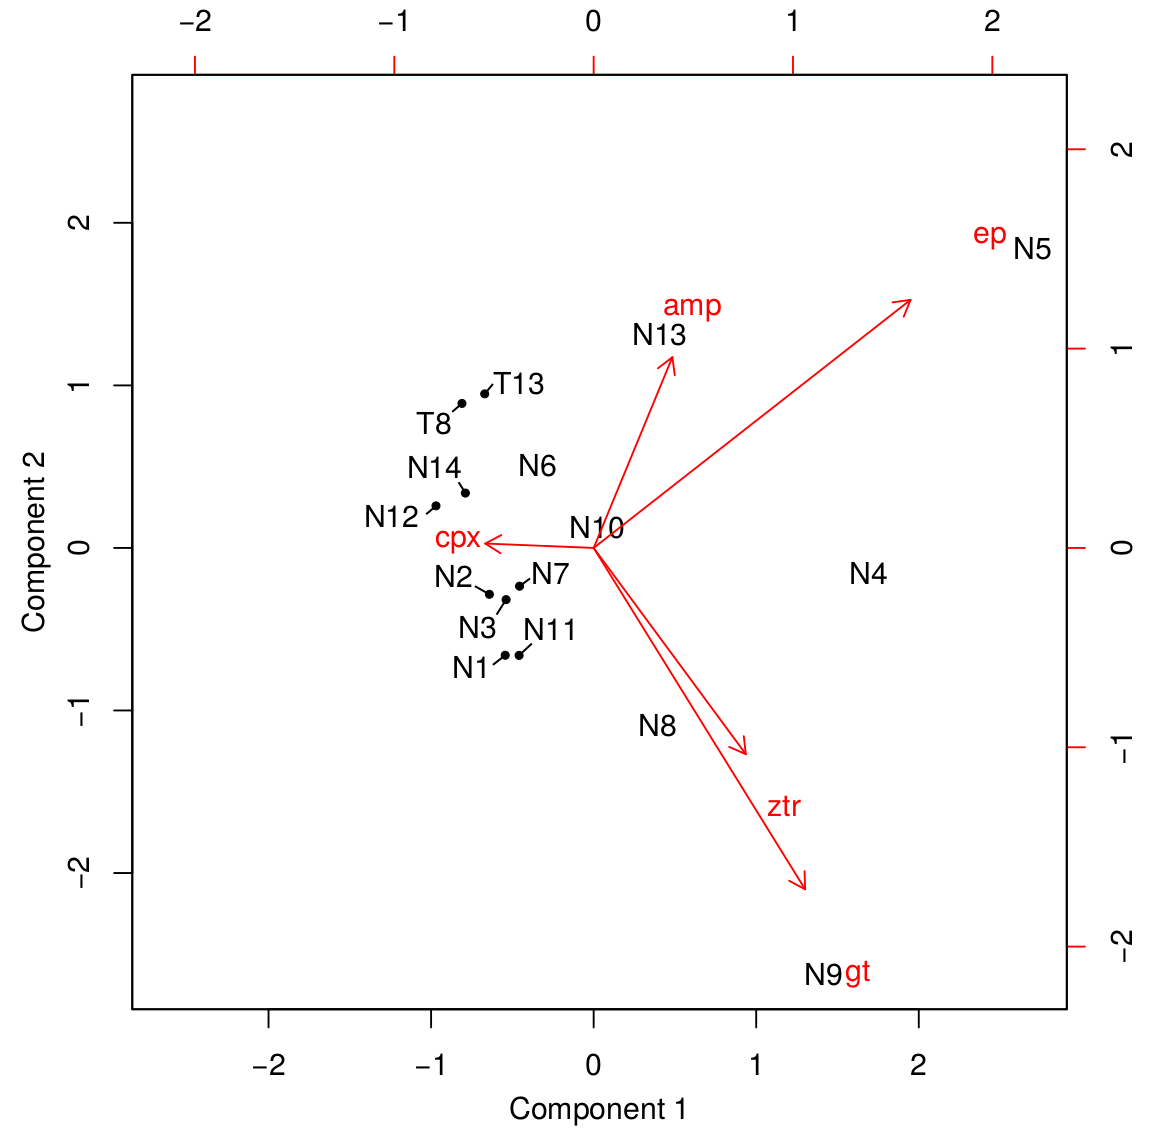
\includegraphics[width=.7\textwidth]{CA.png}
  \caption{Correspondence analysis of heavy mineral compositions from
    Namibia \citep{vermeesch2016a} shown as a biplot.  Samples are
    shown in black, minerals in red.}
  \label{fig:CA}
\end{figure}

\section{Discussion and conclusions}
\label{sec:conclusions}

It is common practice in sedimentary petrography, palaeontology and
palynology to report the relative abundances of minerals, fossils or
pollen as percentages. Unfortunately, by doing so one loses the
ability to quantify the statistical uncertainty of the underlying
point-counting data.  Normalisation of point-counts also compromises
the ability to deal with missing (zero) components.\\

The statistical methods reviewed in this paper are built on the
recognition that point-counts represent a distinct class of data.
This new data class shares aspects with, but is fundamentally
different from \citet{aitchison1986}'s compositional
data. Compositional data only carry relative information
\citep{pawlowsky2011}, and the absolute abundances of their components
are irrelevant. In stark contrast with this, for point-counting data
the absolute abundances \emph{do} matter, because they control the
precision of the estimated compositions \citep{bloemsma2015}.\\

This observation leads to a first recommendation, which is to report
the total number of counts for each sample in published data
tables. This allows the recovery of the raw point-counting data. Those
data can then be further analysed using the techniques introduced in
this paper.\\

Compositional data and point-counting data are closely related to each
other.  In fact, point-counting \emph{data} are underlain by
compositional \emph{populations}. These populations can be constrained
using a combination of multinomial and logratio statistics.\\

If the data are underlain by a single, fixed composition, then the
point-counting data follow a multinomial distribution. In this case,
the fixed composition of the underlying population can be estimated by
pooling all the data together (Section~\ref{sec:pooled}). However,
this simple scenario rarely occurs in the real world.  Provided that a
dataset is large enough, virtually all populations are overdispersed
with respect to the multinomial point-counting uncertainties
(Section~\ref{sec:X2}).\\

For two-component systems, the degree of overdispersion can be
visually assessed on a radial plot (Section~\ref{sec:radial}). The
dispersion may then be quantified using a three parameter continuous
mixture model (Section~\ref{sec:randomeffects}), which can be
generalised to three (or more) components
(Section~\ref{sec:ternary}). The continuous mixture model assumes that
the point-counting data are underlain by a logistic normal
distribution.  Although more realistic than the homogeneous population
assumed by the pooled composition, the continuous mixture model is
still a very simple approximation to real geological scenarios.\\

Correspondence Analysis was introduced as an effective tool for
exploratory analysis of more complex and higher dimensional datasets
(Section~\ref{sec:CA}).  It does not seek to capture the data in a
simplified analytical form.  Instead, CA distills the salient
similarities and differences between samples as a two-dimensional
`map', and which the variables can also be shown. Such biplots can
provide valuable geological insights that would be difficult to obtain
otherwise.\\

CA is closely related to Principal Component Analysis. PCA can be
applied to compositional data and uses Aitchison's Euclidean
logratio-distance as a measure to compare the (dis)similarities
between samples.  In contrast, CA uses the chi-square distance
(Equation~\ref{eq:dij}), which makes it immune to the zero-count
problem. Once we recognise the close affinity between the Aitchison
distance and compositional data on the one hand, and between the
chi-square distance and point-counting data on the other hand, then it
is possible to add further complexity to our statistical analysis.\\

For example, \citet{vermeesch2015} introduce a technique called 3-way
multidimensional scaling to combine different datasets together for
the purpose of sedimentary provenance analysis. Using the insights
gained from this paper, we could use the Aitchison distance to compare
the major and trace element compositions of different samples, and the
chi-square distance to compare their bulk petrography and heavy
mineral counts.

\section*{Acknowledgments}

The methods presented in this paper follow from the work of Rex
Galbraith, who is gratefully acknowledged for patiently answering
numerous questions from the author.  Gert-Jan Weltje and an anonymous
reviewer are thanked for their constructive comments on the submitted
manuscript.

%\bibliographystyle{elsarticle-num.bst}
%\bibliographystyle{/home/pvermees/Dropbox/abbrvplainnat.bst}
%\bibliography{/home/pvermees/Dropbox/biblio}

\begin{thebibliography}{32}
\providecommand{\natexlab}[1]{#1}
\providecommand{\url}[1]{\texttt{#1}}
\expandafter\ifx\csname urlstyle\endcsname\relax
  \providecommand{\doi}[1]{doi: #1}\else
  \providecommand{\doi}{doi: \begingroup \urlstyle{rm}\Url}\fi

\bibitem[Aitchison(1982)]{aitchison1982}
Aitchison, J.
\newblock The statistical analysis of compositional data.
\newblock \emph{Journal of the Royal Statistical Society}, 44:\penalty0
  139--177, 1982.

\bibitem[Aitchison(1983)]{aitchison1983}
Aitchison, J.
\newblock Principal component analysis of compositional data.
\newblock \emph{Biometrika}, 70\penalty0 (1):\penalty0 57--65, 1983.
\newblock \doi{10.1093/biomet/70.1.57}.

\bibitem[Aitchison(1986)]{aitchison1986}
Aitchison, J.
\newblock \emph{The statistical analysis of compositional data}.
\newblock London, Chapman and Hall, 1986.

\bibitem[Aitchison and Greenacre(2002)]{aitchison2002}
Aitchison, J. and Greenacre, M.
\newblock Biplots of compositional data.
\newblock \emph{Journal of the Royal Statistical Society: Series C (Applied
  Statistics)}, 51\penalty0 (4):\penalty0 375--392, 2002.

\bibitem[Barkley(1934)]{barkley1934}
Barkley, F.~A.
\newblock The statistical theory of pollen analysis.
\newblock \emph{Ecology}, 15\penalty0 (3):\penalty0 283--289, 1934.

\bibitem[Berger and Diester-Haass(1988)]{berger1988}
Berger, W. and Diester-Haass, L.
\newblock Paleoproductivity: the benthic/planktonic ratio in foraminifera as a
  productivity index.
\newblock \emph{Marine Geology}, 81\penalty0 (1-4):\penalty0 15--25, 1988.

\bibitem[Bloemsma and Weltje(2015)]{bloemsma2015}
Bloemsma, M.~R. and Weltje, G.~J.
\newblock {Reduced-rank approximations to spectroscopic and compositional data:
  A universal framework based on log-ratios and counting statistics}.
\newblock \emph{Chemometrics and Intelligent Laboratory Systems}, 142:\penalty0
  206--218, 2015.

\bibitem[Buzas(1990)]{buzas1990}
Buzas, M.~A.
\newblock Another look at confidence limits for species proportions.
\newblock \emph{Journal of Paleontology}, 64\penalty0 (5):\penalty0 842--843,
  1990.

\bibitem[Clark(1982)]{clark1982}
Clark, R.~L.
\newblock Point count estimation of charcoal in pollen preparations and thin
  sections of sediments.
\newblock \emph{Pollen et spores}, 1982.

\bibitem[Dryden(1931)]{dryden1931}
Dryden, A.
\newblock Accuracy in percentage representation of heavy mineral frequencies.
\newblock \emph{Proceedings of the National Academy of Sciences}, 17\penalty0
  (5):\penalty0 233--238, 1931.

\bibitem[Fatela and Taborda(2002)]{fatela2002}
Fatela, F. and Taborda, R.
\newblock Confidence limits of species proportions in microfossil assemblages.
\newblock \emph{Marine Micropaleontology}, 45\penalty0 (2):\penalty0 169--174,
  2002.

\bibitem[Galbraith(2005)]{galbraith2005}
Galbraith, R.~F.
\newblock \emph{Statistics for fission track analysis}.
\newblock CRC Press, 2005.

\bibitem[Galbraith(1988)]{galbraith1988}
Galbraith, R.
\newblock Graphical display of estimates having differing standard errors.
\newblock \emph{Technometrics}, 30\penalty0 (3):\penalty0 271--281, 1988.

\bibitem[Galbraith and Laslett(1993)]{galbraith1993}
Galbraith, R. and Laslett, G.
\newblock Statistical models for mixed fission track ages.
\newblock \emph{Nuclear tracks and radiation measurements}, 21\penalty0
  (4):\penalty0 459--470, 1993.

\bibitem[Greenacre(2005)]{greenacre2005}
Greenacre, M.
\newblock Weighted metric multidimensional scaling.
\newblock In \emph{New developments in classification and data analysis}, pages
  141--149. Springer, 2005.

\bibitem[Greenacre(1984)]{greenacre1984}
Greenacre, M.~J.
\newblock Theory and applications of correspondence analysis.
\newblock page 364, 1984.

\bibitem[Heroy et~al.(2003)Heroy, Kuehl, and Goodbred~Jr]{heroy2003}
Heroy, D.~C., Kuehl, S.~A., and Goodbred~Jr, S.~L.
\newblock {Mineralogy of the Ganges and Brahmaputra Rivers: implications for
  river switching and Late Quaternary climate change}.
\newblock \emph{Sedimentary Geology}, 155\penalty0 (3-4):\penalty0 343--359,
  2003.

\bibitem[Herzschuh(2007)]{herzschuh2007}
Herzschuh, U.
\newblock {Reliability of pollen ratios for environmental reconstructions on
  the Tibetan Plateau}.
\newblock \emph{Journal of Biogeography}, 34\penalty0 (7):\penalty0 1265--1273,
  2007.

\bibitem[Kruskal and Wish(1978)]{kruskal1978}
Kruskal, J.~B. and Wish, M.
\newblock \emph{Multidimensional scaling}, volume 07-011 of \emph{Sage
  University Paper series on Quantitative Application in the Social Sciences}.
\newblock Sage Publications, Beverly Hills and London, 1978.

\bibitem[Legendre and Gallagher(2001)]{legendre2001}
Legendre, P. and Gallagher, E.~D.
\newblock Ecologically meaningful transformations for ordination of species
  data.
\newblock \emph{Oecologia}, 129\penalty0 (2):\penalty0 271--280, 2001.

\bibitem[Mart{\'\i}n-Fern{\'a}ndez et~al.(2003)Mart{\'\i}n-Fern{\'a}ndez,
  Barcel{\'o}-Vidal, and Pawlowsky-Glahn]{martin2003}
Mart{\'\i}n-Fern{\'a}ndez, J.~A., Barcel{\'o}-Vidal, C., and Pawlowsky-Glahn,
  V.
\newblock Dealing with zeros and missing values in compositional data sets
  using nonparametric imputation.
\newblock \emph{Mathematical Geology}, 35\penalty0 (3):\penalty0 253--278,
  2003.

\bibitem[Morton and Hallsworth(1994)]{morton1994}
Morton, A.~C. and Hallsworth, C.
\newblock Identifying provenance-specific features of detrital heavy mineral
  assemblages in sandstones.
\newblock \emph{Sedimentary Geology}, 90\penalty0 (3-4):\penalty0 241--256,
  1994.

\bibitem[Patterson and Fishbein(1989)]{patterson1989}
Patterson, R.~T. and Fishbein, E.
\newblock Re-examination of the statistical methods used to determine the
  number of point counts needed for micropaleontological quantitative research.
\newblock \emph{Journal of Paleontology}, 63\penalty0 (2):\penalty0 245--248,
  1989.

\bibitem[Pawlowsky-Glahn and Buccianti(2011)]{pawlowsky2011}
Pawlowsky-Glahn, V. and Buccianti, A.
\newblock \emph{{Compositional data analysis: Theory and applications}}.
\newblock John Wiley \& Sons, 2011.

\bibitem[Pearson(1901)]{pearson1901}
Pearson, K.
\newblock On lines and planes of closest fit to systems of points in space.
\newblock \emph{The London, Edinburgh, and Dublin Philosophical Magazine and
  Journal of Science}, 2\penalty0 (11):\penalty0 559--572, 1901.

\bibitem[Van~der Plas and Tobi(1965)]{vanderplas1965}
Van~der Plas, L. and Tobi, A.
\newblock A chart for judging the reliability of point counting results.
\newblock \emph{American Journal of Science}, 263\penalty0 (1):\penalty0
  87--90, 1965.

\bibitem[Vermeesch(2013)]{vermeesch2013}
Vermeesch, P.
\newblock Multi-sample comparison of detrital age distributions.
\newblock \emph{Chemical Geology}, 341:\penalty0 140--146, 2013.

\bibitem[Vermeesch and Garzanti(2015)]{vermeesch2015}
Vermeesch, P. and Garzanti, E.
\newblock {Making geological sense of `Big Data' in sedimentary provenance
  analysis}.
\newblock \emph{Chemical Geology}, 409:\penalty0 20--27, 2015.

\bibitem[Vermeesch et~al.(2016)Vermeesch, Resentini, and
  Garzanti]{vermeesch2016a}
Vermeesch, P., Resentini, A., and Garzanti, E.
\newblock {An R package for statistical provenance analysis}.
\newblock \emph{Sedimentary Geology}, 2016.

\bibitem[Weltje(2002)]{weltje2002}
Weltje, G.
\newblock Quantitative analysis of detrital modes: statistically rigorous
  confidence regions in ternary diagrams and their use in sedimentary
  petrology.
\newblock \emph{Earth-Science Reviews}, 57\penalty0 (3-4):\penalty0 211 -- 253,
  2002.
\newblock ISSN 0012-8252.
\newblock \doi{DOI: 10.1016/S0012-8252(01)00076-9}.

\bibitem[Wendt and Carl(1991)]{wendt1991}
Wendt, I. and Carl, C.
\newblock The statistical distribution of the mean squared weighted deviation.
\newblock \emph{Chemical Geology: Isotope Geoscience Section}, 86\penalty0
  (4):\penalty0 275--285, 1991.

\bibitem[Weng et~al.(2006)Weng, Hooghiemstra, and Duivenvoorden]{weng2006}
Weng, C., Hooghiemstra, H., and Duivenvoorden, J.~F.
\newblock Challenges in estimating past plant diversity from fossil pollen
  data: statistical assessment, problems, and possible solutions.
\newblock \emph{Diversity and distributions}, 12\penalty0 (3):\penalty0
  310--318, 2006.

\end{thebibliography}


\end{document}
